%!TEX root = ../report.tex

\section{Architectural Patterns}
% From https://en.wikipedia.org/wiki/Architectural_pattern
An architectural pattern is a general, reusable solution to a commonly occurring problem in software architecture within a given context.
Architectural patterns are similar to software design pattern but have a broader scope.
The architectural patterns address various issues in software engineering, such as computer hardware performance limitations, high availability and minimization of a business risk.

A software architecture consists of:
\begin{itemize}
	\item Components (Subsystems)
	\subitem $\rightarrow$ Computational units with specified interface (e.g. filters, databasesm layers, objects)
	\item Connectors (Communication)
	\subitem $\rightarrow$ Interactions between the components (subsystems) (e.g calls, pipes, events, shared data)
\end{itemize}

The following sections list some of the most relevant architectural patterns.
\newpage

\subsection{Layer Pattern}
As the name suggests, the layer pattern consists of layers, which also can be called virtual machines.
A layer is an abstraction that provides a set of attributes and operations.
The lower a layer is, the more specific is its implementation.\newline

\textbf{Advantages of the layer pattern:}
\begin{itemize}[topsep=5pt, itemsep=0pt]
	\item Reusability of Layers, especially in a closed architecture:
		\subitem Black box reuse of layers can reduce development effort and number of defects
	\item Support for standardization:
		\subitem Different implementations of the same interface can be used interchangeable
		\subitem (especially if coupled with the bridge or strategy pattern)
	\item Low Coupling:
		\subitem Changes to hardware, os, database system, user interface
		system, ... only affects one layer
	\item Improved Testability:
		\subitem Closed architecture with hierarchical call hierarchy requires half
		compared to p2p architecture
\end{itemize}

\textbf{Disadvantages of the layer pattern:}
\begin{itemize}[topsep=5pt, itemsep=0pt]
	\item A local change in a lower layer may require rework in higher layers:
	\subitem Example: Changing from 10Mbit/sec Ethernet to 1 Gbit/sec Ethernet
	\item Lower efficiency:
		\subitem Data must be transferred through the intermediate layers, may even have to be
	 transformed
		\subitem Error messages produced in lower levels must be transformed to higher level messages
\end{itemize}

\begin{description}
	\item \textbf{Closed Architecture (Opaque Layering):}
		\subitem $\rightarrow$ Each layer can only call operations from the layer below.
	\item \textbf{Open Architecture (Transparent Layering):}
		\subitem $\rightarrow$ Each layer can call operations from \textbf{any} layer below
\end{description}
\newpage

\begin{figure}[h]
	\centering
	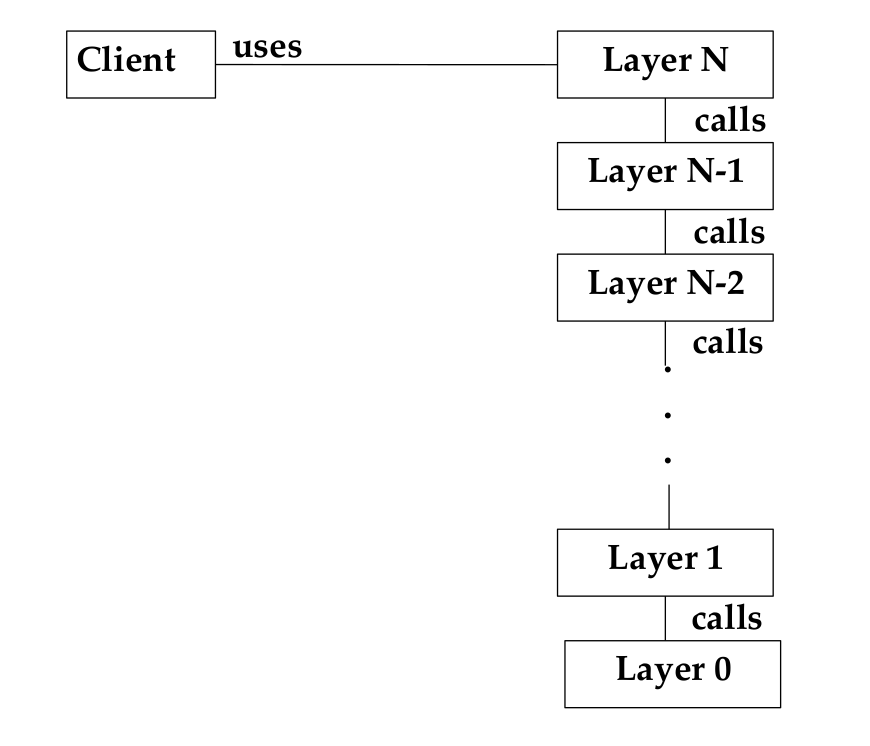
\includegraphics[width=0.6\linewidth]{images/pattern_layer.png}
	\caption{Structure of Layer Pattern}
\end{figure}

\textbf{5 Steps to Create a Layered Architecture}
\begin{enumerate}
  \item Identify subsystems, specify interface for each layer
  \item Structure the individual layers (bridge and strategy pattern)
  \item Specify the communication protocol between adjacent layers (push/pull)
  \item Decouple adjacent layers (return results only as parameters to upper layers/use callbacks)
  \item Design an error-handling strategy (try handling errors on lowest possible layer)
\end{enumerate}
\newpage


\subsection{Repository Pattern}
The repository pattern is used to support a collection of independent programs that work cooperatively on a common data structure called the repository.
Subsystems access and modify data from a single data structure called the repository.
The subsystems are exchanging data via the repository and are therefore loosely coupled.
The control flow is not specified by the pattern.
This means control flow can be established by the subsystems themselves e.g. through
locks and synchronization primitives.\newline
\begin{figure}[h]
	\centering
	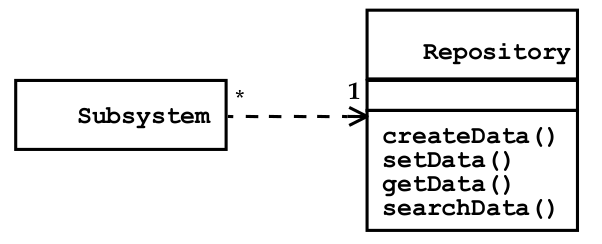
\includegraphics[width=0.7\linewidth]{images/pattern_repository.png}
	\caption{Structure of Repository Pattern}
\end{figure}
\newpage


\subsection{Blackboard Pattern}
This pattern uses knowledge sources which communicate over a \glqq blackboard\grqq \ in order to solve a problem.
The blackboard is the repository for the problem.
Each knowledge source reads the content that is placed on the blackboard, processes it and generates new hypotheses based on the knowledge the source has and places this information back on the blackboard.
A control instance governs the flow of problem-solving activity in the system and notifies sources if new information is placed on the blackboard.

In general, the blackboard pattern is used when no algorithm for the problem is known.
\newline

\textbf{Advantages of the blackboard pattern:}
\begin{itemize}[topsep=5pt, itemsep=0pt]
	\item Problem solving support:
		\subitem Allows problems in domains without closed approaches or infeasible solution space
	\item Changeability and maintainability:
		\subitem Low coupling, strict separation between controller	and data structures in blackboard
	\item Fault tolerance and robustness:
		\subitem Blackboards  are tolerant against noisy data, only hypotheses with strong evidence survive
\end{itemize}

\textbf{Disadvantages of the blackboard pattern:}
\begin{itemize}[topsep=5pt, itemsep=0pt]
	\item Difficulty of testing:
		\subitem Nondeterministic, results are often not reproducible
	\item No solution guaranteed:
		\subitem Cannot solve every problem
	\item Difficulty to establish a good control strategy:
		\subitem Requires an experimental approach
	\item High development effort:
		\subitem Most blackboard systems take years to evolve
\end{itemize}
\newpage

\begin{figure}[h]
	\centering
	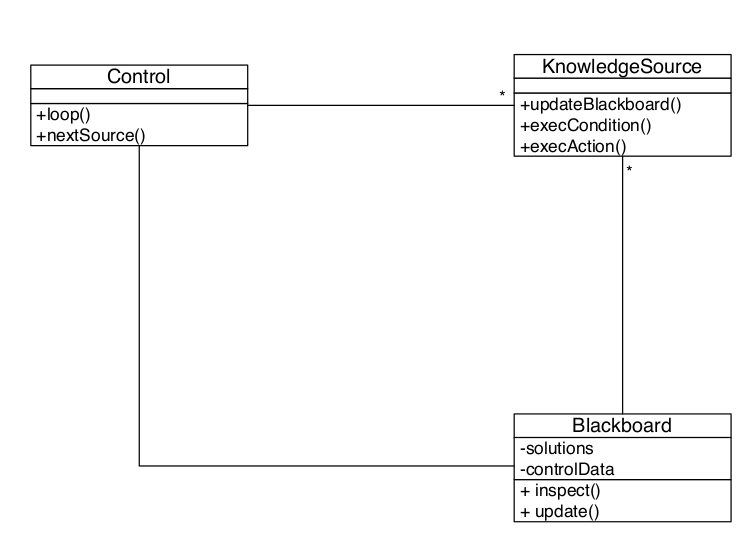
\includegraphics[width=0.85\linewidth]{images/pattern_blackboard.png}
	\caption{Structure of Blackboard Pattern}
\end{figure}

\textbf{6 Steps to Realize a Blackboard Pattern}
\begin{enumerate}
	\item Define the problem (Identify application domain and actors, specify requirements)
	\item Define the solution space (top-level and intermediate)
	\item Identify the knowledge sources (in/-outputs)
	\item Define the blackboard, identify needed representations (knowledge sources may not understand information of each other)
	\item Define the control (Who can construct hypotheses? Who decides about credibility/acceptability?)
	\item Implement the knowledge sources (split into condition part and action part, use computational intelligence or conventional methods)
\end{enumerate}
\newpage

\subsection{Client-Dispatcher-Server Pattern}
The client-dispatcher-server pattern decouples the client from the server.
Usually the client had to know where the server is, now the server is even dynamically interchangeable (server registers to the dispatcher on startup/runtime) what is good for re-configurations and fault tolerance.\\
\begin{minipage}{.5\textwidth}
  Structure:\\
  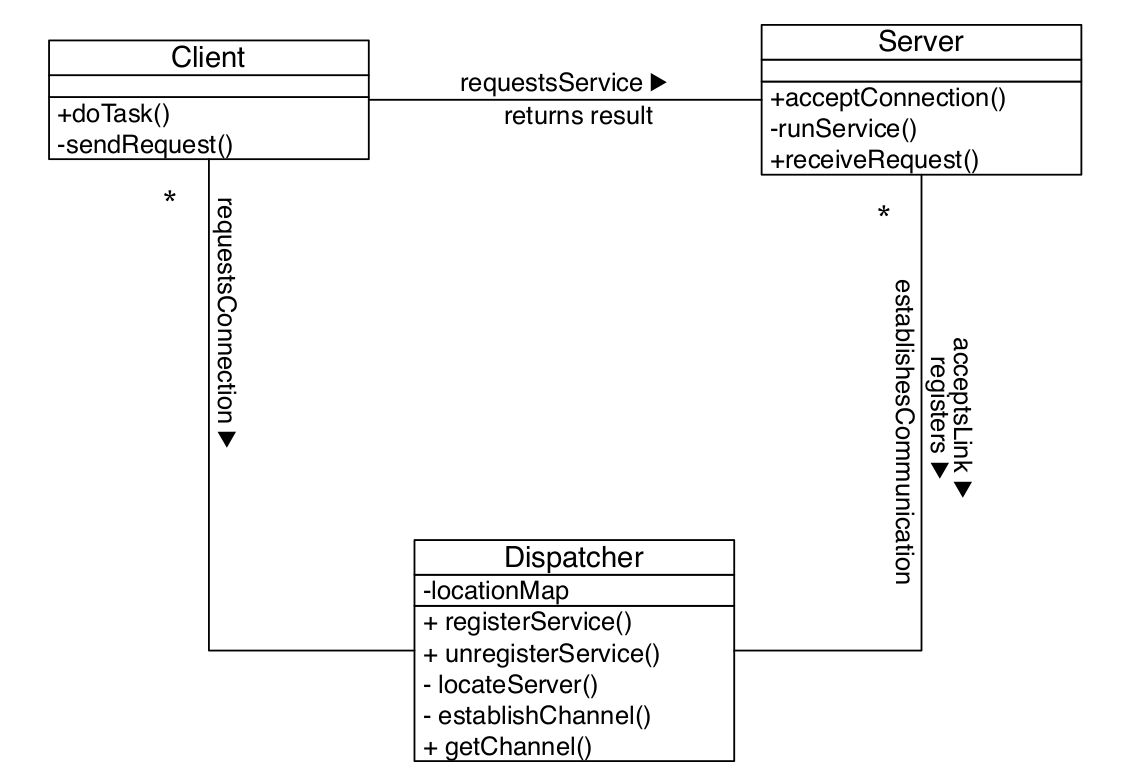
\includegraphics[width=\linewidth]{images/pattern_client_dispatcher_server.png}\\
\end{minipage}
\begin{minipage}{.5\textwidth}
  \vspace{1em}
  Eventflow:\\
  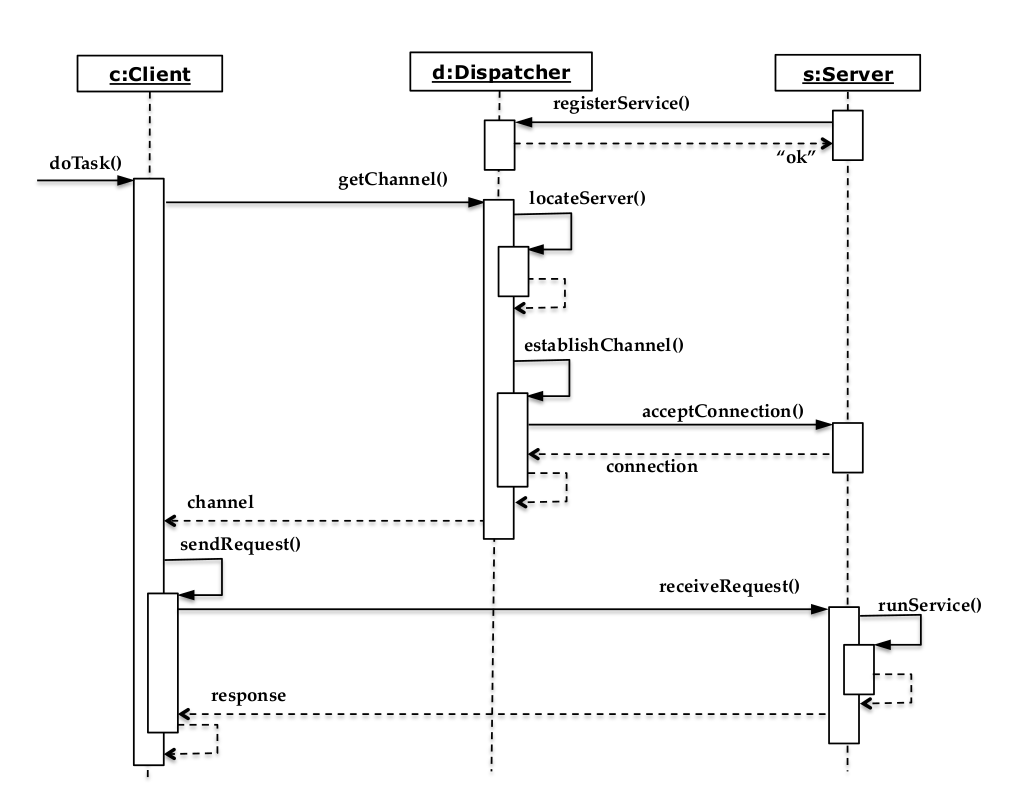
\includegraphics[width=\linewidth]{images/eventflow_client_dispatcher_server.png}
\end{minipage}\\
\\
\textbf{Communication Protocols:}
\begin{description}
  \item[CDprotocol:] Specifies how to ask for servers and handles communication errors.
  \item[DSprotocol:] Specifies how the server registers with the dispatcher and determines the step necessary for a client to establish a connection.
  \item[CSprotocol:] Specifies the communication between client and server.
\end{description}

\textbf{6 Steps to Implement Client-Dispatcher-Server}
\begin{enumerate}
  \item During system design identify the subsystems that act as clients and servers
  \item Decide on the communication mechanism to be used for the protocols (Shared memory, sockets)
  \item Specify the protocols
  \item Decide on a naming scheme for the dispatcher (URLs are ok, IPs not)
  \item Implement the dispatcher
  \begin{enumerate}
    \item Decide how to implement the 3 protocols (sockets, RPM)
    \item Implement requests, responses and errors
    \item Implement a repository that maps server names to addresses
  \end{enumerate}
  \item Implement the client and server (also: when does the server register? Startup or runtime?)
\end{enumerate}
\newpage

\subsection{Broker Pattern}
The broker pattern coordinates the communication between heterogeneous nodes.\\
\\
\textbf{Nonfunctional Requirements:}\\
\vspace{-1.5em}
\begin{description}
  \item[Low Coupling:] Decoupling of service and communication
  \item[Location Transparency:] Services are independent of the server location
  \item[Runtime Extensibility:] Ability to add, remove, exchange components at runtime
  \item[Platform Transparency:] Clients and servers can be written in different languages.
\end{description}
Structure:\\
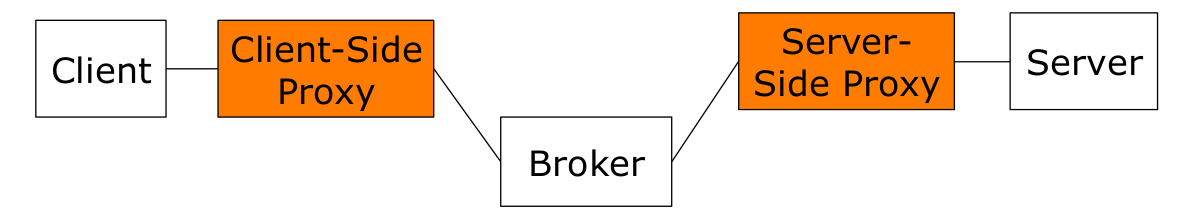
\includegraphics[width=\linewidth]{images/pattern_broker.png}
\textbf{Client-Side Proxy:} Lets the remote object appear as local one, hides the inter-process communication details used for message transfer between client and broker and provides (un-)marshalling/(de-)serialization of parameters and results.\\
\textbf{Server-Side Proxy:} Same as Client-Side proxy only for the server.\\
Eventflow:\\
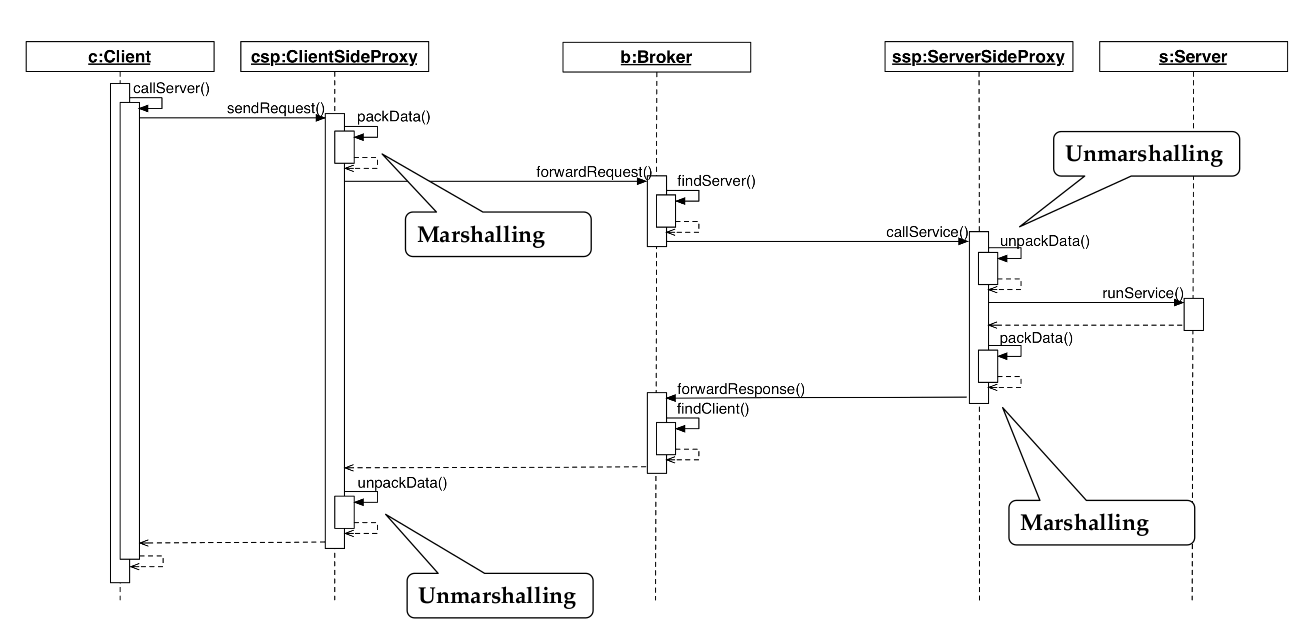
\includegraphics[width=\linewidth]{images/eventflow_broker.png}
\textbf{Steps to Realize a Broker Pattern:}
\begin{enumerate}
  \item Provide the object model and service definitions.
  \item Define the broker service.
  \item Implement the broker component and proxy object at the client and server side.
  \item Implement the client and server.
\end{enumerate}


\newpage
